%!TEX TS-program = xelatex
%!TEX TS-options = -synctex=1
%!TEX encoding = UTF-8 Unicode
%
%  handout
%
%  Created by Mark Eli Kalderon on 2010-10-26.
%  Copyright (c) 2010. All rights reserved.
%

\documentclass[12pt]{article} 

% Definitions
\newcommand\myauthor{Mark Eli Kalderon} 
\newcommand\mytitle{Audition, Vision, and Time}

% Packages
\usepackage{geometry} \geometry{a4paper}
\usepackage{graphicx}

% XeTeX
\usepackage{fontspec}
\usepackage{xltxtra,xunicode}
\defaultfontfeatures{Scale=MatchLowercase,Mapping=tex-text}
\setmainfont{Hoefler Text}

% Bibliography
\usepackage[round]{natbib} 

% Title Information
\title{\mytitle}
\author{\myauthor}
\date{}

%%% BEGIN DOCUMENT
\begin{document}

% Title Page
\maketitle
\vskip 2em \hrule height 0.4pt \vskip 2em
% Main Content

% Layout Settings
\setlength{\parindent}{1em}

\begin{center}
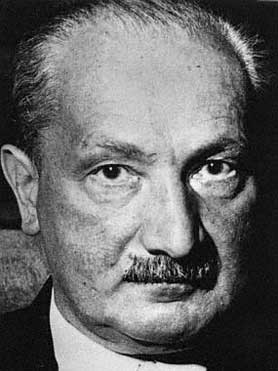
\includegraphics[height=3cm]{heidegger.jpeg} 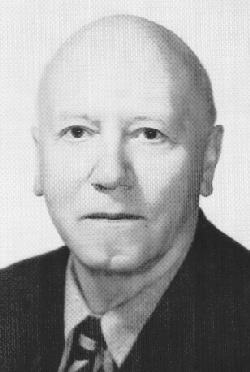
\includegraphics[height=3cm]{broad.jpg}
\end{center}

\begin{quote}
    We never really first perceive a throng of sensations, e.g., tones and noises, in the appearance of things \ldots; rather we hear the storm whistling in the chimney, we hear the three-motored plane, we hear the Mercedes in immediate distinction from the Volkswagen. Much closer to us than all sensations are the things themselves. We hear the door shut in the house and never hear acoustical sensations or even mere sounds. In order to hear a bare sound we have to listen away from things, divert our ears from them, i.e., listen abstractly. ---\emph{Heidegger,1935, ``The Origin of a Work of Art''}
\end{quote}

\begin{quote}
	In its purely phenomenological aspect \emph{seeing} is ostensibly \emph{saltatory}. It seems to leap the spatial gap between the percipient's body and a remote region of space. Then again, it is ostensibly \emph{prehensive} of the surfaces of distant bodies as coloured and extended, and of external events as colour-occurrences \emph{localized} in remote regions of space. In its purely phenomenological aspect \emph{hearing} is ostensibly prehensive, not of bodies, but only of events or processes as occurrences of sound qualities. It is not ostensibly saltatory, for these events or processes are not heard as localized in remote restricted regions of space. They are heard rather as emanating from remote centres and pervading with diminishing intensity the surrounding space. ---\emph{Broad, 1951, ``Some Elementary Reflections on Sense-Perception''}
\end{quote}


\end{document}